\documentclass[11pt]{article}
\usepackage{amssymb}
\usepackage{amsmath}
\usepackage{amsthm}
\usepackage{fullpage}
\usepackage{hyperref}
\usepackage{multicol}
\usepackage{svg}
\usepackage[h]{esvect}
\usepackage{graphicx}
\usepackage{tikz}
\usepackage{pgfplots}
\usetikzlibrary{arrows.meta}
\usepackage{gensymb}
\setlength{\parskip}{1ex}
\setlength{\parindent}{0pt}
\def\N {{\mathbb N}}
\def\Z {{\mathbb Z}}
\def\R {{\mathbb R}}
\def\comp {{\mathrm{comp}}}
\def\proj {{\mathrm{proj}}}
\def\Grad {\mathrm{grad\,}}
\def\Div {\mathrm{div\,}}
\def\Curl {\mathrm{curl\,}}
\newcommand{\partialderiv}[2] {\frac{\partial #1}{\partial #2}}
\newcommand{\Implies}{\mbox{ IMPLIES }}
\newcommand{\Or}{\mbox{ OR }}
\renewcommand{\And}{\mbox{ AND }}
\newcommand{\Not}{\mbox{NOT}}
\newcommand{\Iff}{\mbox{ IFF }}
\newcommand{\True}{\mbox{T}}
\newcommand{\False}{\mbox{F}}
\newcommand{\norm}[1]{\lVert #1 \rVert}
\usepackage{listings}
\usepackage{xcolor}

\definecolor{codegreen}{HTML}{237e02}
\definecolor{codegray}{rgb}{0.5,0.5,0.5}
\definecolor{codepurple}{HTML}{8F4673}
\definecolor{codebrown}{HTML}{ce9178}
\definecolor{codecyan}{HTML}{098658}
\lstdefinestyle{pythonstyle}{
    commentstyle=\color{codegreen},
    keywordstyle=\color{codepurple},
    numberstyle=\tiny\color{codegray},
    stringstyle=\color{codebrown},
    basicstyle=\ttfamily\small,
    breakatwhitespace=false,         
    breaklines=true,                 
    captionpos=b,                    
    keepspaces=true,                 
    numbers=none,                    
    numbersep=5pt,                  
    showspaces=false,                
    showstringspaces=false,
    showtabs=false,                  
    tabsize=2
}

\lstset{style=pythonstyle}

\newtheorem{theorem}{Theorem}[section]
\newtheorem{corollary}{Corollary}[theorem]
\newtheorem{lemma}[theorem]{Lemma}
\newtheorem{definition}[theorem]{Definition}
\newcounter{example}[section]
\newenvironment{example}[1][]{\refstepcounter{example}\par\medskip
   \noindent \textbf{Example~\theexample. #1} \rmfamily}{\par \begin{flushright} \textbf{End of Example~\theexample} \end{flushright}}

\begin{document}
\begin{center}

{\bf \Large \bf MATH209 Summer 2021 Tets 2.1}\\
{\bf \large Kevin Gao}
\end{center}

\begin{enumerate}
    \item Question 1
    \begin{enumerate}
        \item
        We begin by finding the partial derivative of $z$ with respect to $x$ and $y$
        $$
        \begin{aligned}
        \partialderiv{z}{x} &= 2x \\
        \partialderiv{z}{y} &= 2y
        \end{aligned}
        $$
        which evaluated at $(1,2,5)$ yields
        $$
        \begin{aligned}
        \left. \partialderiv{z}{x} \right\vert_{x=1,y=2} &= 2 \\
        \left. \partialderiv{z}{y} \right\vert_{x=1,y=2} &= 4.
        \end{aligned}
        $$
        Then, the tangent plane at $(1,2,5)$ is
        $$
        z - 5 = 2(x-1) + 4(y-2)
        $$
        
        \item
        From the equation of the tangent plane, we know that the normal vector is $\vv n = (2,4,-1)$. Then, the line $L$ can be defined as
        $$
        L:\; (1,2,5) + (2,4,-1)t
        $$
        which can be written in parametric form as
        $$
        (1+2t, 2+4t, 5-t)
        $$
        
        \item To find the intersection, set up the following equation
        $$
        \begin{aligned}
            z &= x^2 + y^2 \\
            5-t &= (1+2t)^2 + (2+4t)^2 \\
            5-t &= 1+4t + 4t^2 + 4 + 16t+ 16t^2 \\
            t &= -1.05 \qquad t = 0
        \end{aligned}
        $$
        Hence, the intersection points are
        $$
        (1,2,5) \qquad (-1.1, -2.2, 6.05)
        $$
    \end{enumerate}
    
    \item
    Let $\vv v = (\sqrt3,1)$. Then, the unit vector $\vv u$ in the direction of $\vv v$ is
    $$
    \vv u = \frac{\vv v}{\norm{\vv v}} = \frac{(\sqrt3,1)}{2} = (\sqrt3/2,1/2)
    $$
    Then, the directional derivative can be calculated as the dot product between the gradient of the function and the unit vector $\vv u$
    $$
    \begin{aligned}
        \partial_{\vv u}f(x,y) &= (\sqrt3/2, 1/2) \cdot \nabla f(x,y) \\
        &= (\sqrt3/2, 1/2) \cdot \left( \frac{1}{y\left( \left(\frac{x}{y} \right)^2 +1\right)},\; \frac{1}{y^2 \left( \left(\frac{x}{y} \right)^2 +1\right)} \right) \\
        &= \frac{\sqrt{3}y-x}{2x^2+2y^2}
    \end{aligned}
    $$
    
    \item To find those points, we first find the critical points using first derivative test
    $$
    f_x(x,y) = 4-9x^2-2y^2 \qquad f_y(x,y)=-4xy
    $$
    Setting both equations to zero, we can find the following critical points: $(0,\sqrt2)$, $(\sqrt2/3,0)$, $(0,-\sqrt2)$, and $(-\sqrt2/3,0)$.
    
    To confirm that those points are local min/max, or saddle points, use the second derivative test
    $$
    f_{xx} = -18x \qquad f_{yy} = -4x \qquad f_{xy} = -4y
    $$
    Define $D$ as
    $$
    D(a,b) = f_{xx}(a,b) f_{yy}(a,b) - \left[ f_{xy}(a,b) \right]^2 = 72a^2 - 16b^2
    $$
    \begin{itemize}
        \item $(0,\sqrt2,0)$: $D=-32<0$, saddle point
        \item $(\sqrt2/3,0,1.57)$: $D=16>0$, $f_{xx}(\sqrt2/3,0) < 0$, local maximum
        \item $(0,-\sqrt2,0)$: $D<0$, saddle point
        \item $(-\sqrt2/3,0,-1.57)$: $D=16>0$, $f_{xx}(-\sqrt2/3,0) > 0$, local minimum
    \end{itemize}
    
    \item Question 4
    
    The hyperboloid is defined implicitly by $F(x,y,z)=2x^2+y^2-z^2-1/7=0$. Let $(a,b,c)$ be an arbitrary point on the hyperboloid. In this case, the plane tangent to the hyperboloid at $(a,b,c)$ is given by
    $$
    F_x(a,b,c)(x-a) + F_y(a,b,c)(y-b) + F_z(a,b,c)(z-c) = 0
    $$
    Calculate the partial derivatives with respect to $x,y,z$, respectively. Then the tangent plane at $(a,b,c)$ can be written as
    $$
    4a(x-a) + 2b(y-b) - 2c(z-c) = 0
    $$
    whose normal is $(4a,2b,-2c)$. Suppose that the tangent plane is parallel to the plane $2z=2x-3y$, which implies that there exists some scalar $k$ such that
    $$
    (4a,2b,-2c) = k(2,-3,-2)
    $$
    This implies that $a=1/2k$, $b=-3/2k$, $c=k$. Since $(a,b,c)$ must be on the hyperboloid,
    $$
    2a^2 + b^2 - c^2 - \frac{1}{7} = 0
    $$
    Substitute $k$
    $$
    \begin{aligned}
        2\left(\frac{1}{2}k\right)^2 + \left(-\frac32k\right)^2 - k ^2 - 1/7 &= 0 \\
        k &= \pm 0.286
    \end{aligned}
    $$
    Then, $a=1/2k = \pm 0.143$, $b=-3/2k= \mp 0.429$, $c= \pm 0.286$
    
    Hence, the the tangent plane that is parallel to $2z=2x-3y$ is tangent to the hyperboloid at $(0.143,-0.429,0.286)$ and $(-0.143,0.429,-0.286)$.
    
    \item Question 5
    \begin{enumerate}
        \item 
        $$
        \begin{aligned}
            \partialderiv{z}{r} &= \partialderiv{z}{x}\partialderiv{x}{r} + \partialderiv{z}{y}\partialderiv{y}{r} \\
            &= \partialderiv{z}{x} (\cos\theta) + \partialderiv{z}{y} (\sin\theta)
        \end{aligned}
        $$
        \item
        $$
        \begin{aligned}
            \partialderiv{z}{\theta} &= \partialderiv{z}{x}\partialderiv{x}{\theta} + \partialderiv{z}{y}\partialderiv{y}{\theta} \\
            &= \partialderiv{z}{x} (-r\sin\theta) + \partialderiv{z}{y} (r\cos\theta)
        \end{aligned}
        $$
        \item
        Consider the left hand side (LHS) of the expression. To show that this is an identity, we want to show that LHS equals RHS
        $$
        \begin{aligned}
            \left( \partialderiv{z}{r} \right)^2 =
            \left(\partialderiv{z}{x}\right)^2 (\cos^2\theta) + 2\partialderiv{z}{x}\partialderiv{z}{y}\cos\theta\sin\theta + \left(\partialderiv{z}{y}\right)^2 (\sin^2\theta)
        \end{aligned}
        $$
        $$
        \begin{aligned}
            \left( \partialderiv{z}{\theta} \right)^2 &= \frac{1}{r^2} \left[ \left(\partialderiv{z}{x}\right)^2 (r^2\sin^2\theta) -\frac{2}{r^2}\partialderiv{z}{x}\partialderiv{z}{y}\cos\theta\sin\theta + \left(\partialderiv{z}{y}\right)^2 (r^2\cos^2\theta) \right] \\
            &= \left(\partialderiv{z}{x}\right)^2 (\sin^2\theta) -2\partialderiv{z}{x}\partialderiv{z}{y}\cos\theta\sin\theta + \left(\partialderiv{z}{y}\right)^2 (\cos^2\theta)
        \end{aligned}
        $$
        Hence,
        $$
        \begin{aligned}
            \left( \partialderiv{z}{r} \right)^2 + \left( \partialderiv{z}{\theta} \right)^2 &= \left(\partialderiv{z}{x}\right)^2 (\cos^2\theta) +  \left(\partialderiv{z}{y}\right)^2 (\sin^2\theta) + \left(\partialderiv{z}{x}\right)^2 (\sin^2\theta) + \left(\partialderiv{z}{y}\right)^2 (\cos^2\theta) \\
            &= \left(\partialderiv{z}{x}\right)^2 (\cos^2\theta+\sin^2\theta) + \left(\partialderiv{z}{y}\right)^2 (\cos^2\theta+\sin^2\theta)
        \end{aligned}
        $$
        By trigonometry identity (Pythagorean's identiy $\sin^2\theta+\cos^2\theta=1$),
        $$
        \left( \partialderiv{z}{r} \right)^2 + \left( \partialderiv{z}{\theta} \right)^2 = \left(\partialderiv{z}{x}\right)^2 + \left(\partialderiv{z}{y}\right)^2 = RHS
        $$
        Hence $LHS=RHS$, the expression is an identity.
    \end{enumerate}
    
    \item Question 6
    
    Let $x,y,z$ be the dimensions of the box. Since the volume of the box is $500$, we can rewrite $z=\frac{500}{xy}$.
    
    We want to minimize the surface area of the box
    $$
    f(x,y) = xy+2y\frac{500}{xy}+2x\frac{500}{xy} = xy+\frac{1000}{x}+\frac{1000}{y}
    $$
    whose first-order partial derivatives are
    $$
    f_x(x,y) = y-\frac{1000}{x^2} \qquad f_y(x,y) = x-\frac{1000}{y^2}
    $$
    Solve $f_x(x,y)=f_y(x,y)$ for all positive solutions since dimensions cannot be negative.
    $$
    x=10 \qquad y=10 \qquad z=5
    $$
    To confirm that they are actual local minimums, use the second derivative test
    $$
    f_{xx} = \frac{2000}{x^3} \qquad f_{yy} = \frac{2000}{y^3} \qquad f_{xy}= 1
    $$
    and
    $$
    D(x,y) = \frac{2000^2}{x^3y^3} - 1
    $$
    Since $D(10,10)>0$ and $f_{xx}(10,10)>0$, $f(10,10)$ is a local minimum.
    
    \item Question 7
    
    The domain of the function
    $$
    f(x,y) = \frac{\ln(x^2+y^2-100)}{(x+y)\sqrt{-xy}}
    $$
    The denominator cannot be zero, hence
    $$
    x+y \neq 0 \qquad \sqrt{-xy} \neq 0
    $$
    The expression inside the square root must be greater than or equal to 0
    $$
    -xy \geq 0
    $$
    The expression inside the logarithm must be greater than 0, hence
    $$
    (x^2+y^2-100)>0
    $$
    


    \tikzset{every picture/.style={line width=0.75pt}} %set default line width to 0.75pt        
    
    \begin{center}
        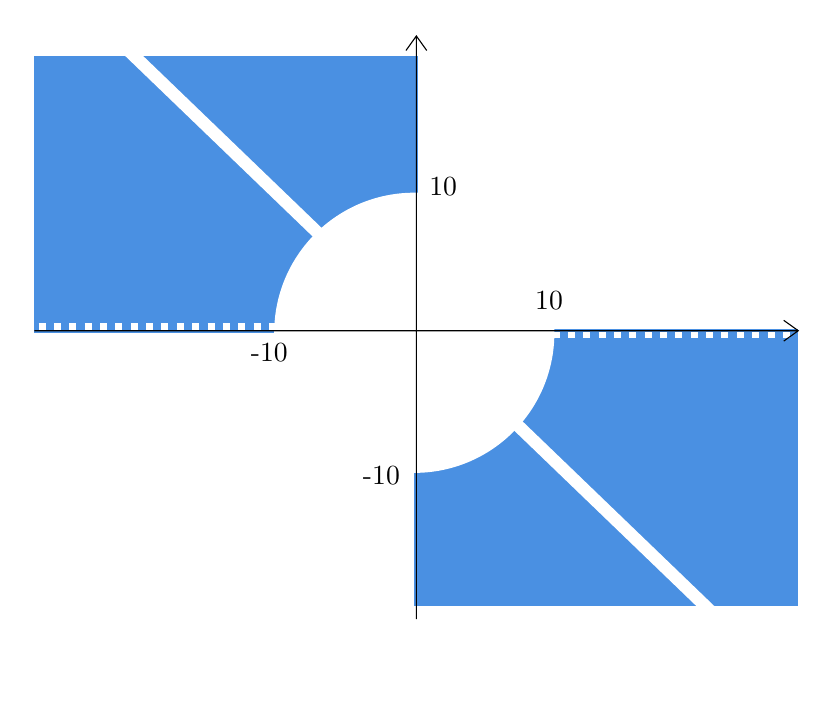
\begin{tikzpicture}[x=0.75pt,y=0.75pt,yscale=-1,xscale=1]
        %uncomment if require: \path (0,300); %set diagram left start at 0, and has height of 300
        
        %Shape: Rectangle [id:dp2280097145973694] 
        \draw  [draw opacity=0][fill={rgb, 255:red, 74; green, 144; blue, 226 }  ,fill opacity=1 ] (128,20.5) -- (496,20.5) -- (496,285.5) -- (128,285.5) -- cycle ;
        %Shape: Rectangle [id:dp3140692587781324] 
        \draw  [draw opacity=0][fill={rgb, 255:red, 255; green, 255; blue, 255 }  ,fill opacity=1 ] (125,154) -- (311,154) -- (311,296) -- (125,296) -- cycle ;
        %Shape: Rectangle [id:dp8856656470121611] 
        \draw  [draw opacity=0][fill={rgb, 255:red, 255; green, 255; blue, 255 }  ,fill opacity=1 ] (313,10) -- (499,10) -- (499,152) -- (313,152) -- cycle ;
        %Shape: Circle [id:dp5132199220051774] 
        \draw  [draw opacity=0][fill={rgb, 255:red, 255; green, 255; blue, 255 }  ,fill opacity=1 ] (243.5,154) .. controls (243.5,116.72) and (273.72,86.5) .. (311,86.5) .. controls (348.28,86.5) and (378.5,116.72) .. (378.5,154) .. controls (378.5,191.28) and (348.28,221.5) .. (311,221.5) .. controls (273.72,221.5) and (243.5,191.28) .. (243.5,154) -- cycle ;
        %Straight Lines [id:da9300856747603725] 
        \draw [color={rgb, 255:red, 255; green, 255; blue, 255 }  ,draw opacity=1 ][line width=4.5]    (165,10) -- (490,323) ;
        %Straight Lines [id:da2711850663330513] 
        \draw [color={rgb, 255:red, 255; green, 255; blue, 255 }  ,draw opacity=1 ][line width=2.25]  [dash pattern={on 2.53pt off 3.02pt}]  (130,151) -- (313,151) ;
        %Straight Lines [id:da16341687310171915] 
        \draw [color={rgb, 255:red, 255; green, 255; blue, 255 }  ,draw opacity=1 ][line width=2.25]  [dash pattern={on 2.53pt off 3.02pt}]  (311,155) -- (494,155) ;
        %Shape: Axis 2D [id:dp887890017377672] 
        \draw  (128,153) -- (496,153)(312,11) -- (312,292) (489,148) -- (496,153) -- (489,158) (307,18) -- (312,11) -- (317,18)  ;
        
        % Text Node
        \draw (231,158) node [anchor=north west][inner sep=0.75pt]   [align=left] {\mbox{-}10};
        % Text Node
        \draw (317,78) node [anchor=north west][inner sep=0.75pt]   [align=left] {10};
        % Text Node
        \draw (368,133) node [anchor=north west][inner sep=0.75pt]   [align=left] {10};
        % Text Node
        \draw (285,217) node [anchor=north west][inner sep=0.75pt]   [align=left] {\mbox{-}10};
        
        
        \end{tikzpicture}
    \end{center}
    The blue region indicates the domain. It contains the second and fourth quadrant excluding: the diagonal line $y=-x$, a circle of radius $10$ centered at $(0,0)$, and the $x$-axis.
    
    \item Question 8
    \begin{enumerate}
        \item Define the function
        $$
        f(x,y) = \sqrt{(3+x)^2 + 4 + (6-y)^2}
        $$
        \item Find the tangent plane
        $$
        f_x(0,0) = \frac{3}{7} \qquad f_y(0,0) = -\frac{6}{7}
        $$
        Then, the tangent plane is
        $$
        z-7 = \frac{3}{7}x - \frac{6}{7}y
        $$
        \item
        $$
        \sqrt{(3.015)^2+4+(5.9919)^2} = f(0.015,0.0081) \approx \frac{3}{7}\cdot 0.015 - \frac{6}{7}\cdot 0.0081 + 7 \approx 6.999485714 
        $$
        The actual value is
        $$
        \sqrt{(3.015)^2+4+(5.9919)^2} \approx 6.999506455
        $$
    \end{enumerate}
    
    \item Question 9
    \begin{enumerate}
        \item Compute the limit as $(x,y)\to(0,0)$ along the $x$-axis
        $$
        f(x,y) \to 0 \qquad \text{as} \qquad (x,y)\to(0,0)\text{ along $y=0$}
        $$
        Meanwhile, if we approach $(x,y)\to(0,0)$ along $y=x^4$
        $$
        f(x,y)=f(x,x^2) = \frac{2x^4x^4}{x^8+\left(x^4\right)^2} = \frac{2x^8}{2x^8} =1
        $$
        Since different path leads to different values, the limit does not exist.
        
        \item
        $$
        \begin{aligned}
            \lim_{(x,y)\to(0,0)} \frac{6x+4\sqrt{x}-6y-4\sqrt{y}}{2\sqrt{x}-2\sqrt{y}} &= \frac{6(x-y)+4(\sqrt{x}-\sqrt{y})}{2(\sqrt{x}-\sqrt{y})} \\
            &= \lim_{(x,y)\to(0,0)}\frac{6(x-y)}{2(\sqrt{x}-\sqrt{y})} + \frac{4(\sqrt{x}-\sqrt{y})}{2(\sqrt{x}-\sqrt{y})} \\
            &= \lim_{(x,y)\to(0,0)}3(\sqrt{x}+\sqrt{y}) + 2 \\
            &= 2
        \end{aligned}
        $$
    \end{enumerate}
    
    \item Question 10
    \begin{enumerate}
        \item
        
        The surface is defined implicitly by
        $$
        F(x,y,z) = \sqrt x + \sqrt y + \sqrt z - \sqrt c = 0
        $$
        The tangent plane is defined by
        $$
        F_x(x_0,y_0,z_0)(x-x_0) + F_y(x_0,y_0,z_0)(y-y_0) + F_z(x_0,y_0,z_0)(z-z_0) = 0
        $$
        Evaluate the partial derivatives and substitute into the expression of the tangent plane.
        $$
        \frac{1}{2}x_0^{-1/2}(x-x_0) + \frac{1}{2}y_0^{-1/2}(y-y_0) + \frac{1}{2}y_0^{-1/2}(y-y_0) = 0
        $$
        
        \item 
        
        Intersection with $x$-axis:
        $$
        \begin{aligned}
            \frac{1}{2}x_0^{-1/2}(x-x_0) + \frac{1}{2}y_0^{-1/2}(0-y_0) + \frac{1}{2}y_0^{-1/2}(0-y_0) &= 0 \\
            x_0^{-1/2}(x-x_0) &= (y_0^{1/2}+z_0^{1/2}) \\
            x &= \frac{x_0^{1/2}+y_0^{1/2}+z_0^{1/2}}{x_0^{-1/2}}
        \end{aligned}
        $$
        Hence
        $$
        \begin{aligned}
            M_x &= \frac{x_0^{1/2}+y_0^{1/2}+z_0^{1/2}}{x_0^{-1/2}}
        \end{aligned}
        $$
        
        Intersection with $y$-axis:
        $$
        \begin{aligned}
            M_y &= \frac{x_0^{1/2}+y_0^{1/2}+z_0^{1/2}}{y_0^{-1/2}}
        \end{aligned}
        $$
        
        Intersection with $y$-axis:
        $$
        \begin{aligned}
            M_z &= \frac{x_0^{1/2}+y_0^{1/2}+z_0^{1/2}}{z_0^{-1/2}}
        \end{aligned}
        $$
        
        \item
        $$
        \begin{aligned}
            M_x+M_y+M_y &= \frac{x_0^{1/2}+y_0^{1/2}+z_0^{1/2}}{x_0^{-1/2}} + \frac{x_0^{1/2}+y_0^{1/2}+z_0^{1/2}}{y_0^{-1/2}} + \frac{x_0^{1/2}+y_0^{1/2}+z_0^{1/2}}{z_0^{-1/2}} \\
            &= \sqrt{x} (\sqrt{x}+\sqrt{y}+\sqrt{z}) + \sqrt{y} (\sqrt{x}+\sqrt{y}+\sqrt{z}) + \sqrt{z} (\sqrt{x}+\sqrt{y}+\sqrt{z}) \\
            &= x + \sqrt{xy} + \sqrt{xz} + y + \sqrt{xy} + \sqrt{yz} + z + \sqrt{xz} + \sqrt{yz} \\
            &= (\sqrt{x}+\sqrt{y}+\sqrt{z})^2 \\
            &= (\sqrt{c})^2 \\
            &= c
        \end{aligned}
        $$
    \end{enumerate}
    
    \item Question 11
    
    $$
    \partialderiv{z}{x} = \frac{e^x}{e^x+e^y} \qquad \frac{\partial^2z}{\partial x^2} = \frac{e^{x+y}}{(e^x+e^y)^2}
    $$
    $$
    \partialderiv{z}{y} = \frac{e^y}{e^x+e^y} \qquad \frac{\partial^2z}{\partial y^2} = \frac{e^{x+y}}{(e^x+e^y)^2}
    $$
    And
    $$
    \frac{\partial^2z}{\partial x \partial y} = \partialderiv{}{y}\partialderiv{z}{x} = \frac{-e^{x+y}}{(e^x+e^y)^2}
    $$
    Hence
    $$
    \begin{aligned}
        \partialderiv{z}{x}\partialderiv{z}{y} - \left( \frac{\partial^2z}{\partial x \partial y} \right) &= \left(\frac{e^{x+y}}{(e^x+e^y)^2}\right)^2 - \left(\frac{-e^{x+y}}{(e^x+e^y)^2}\right)^2 \\
        &= 0
    \end{aligned}
    $$
    Hence, function $z(x,y)=\ln(e^x+e^y)$ is a solution to the partial differential equation.
    
    \item Question 12
    
    At $P=(2,1,3)$,
    $$
    r_1(0) = (2,1,3) \qquad r_2(1) = (2,1,3)
    $$
    Find the tangent vector of the curves $r_1,r_2$ at $t=0, u=1$, respectively.
    $$
    r_1'(t) = (3,-2t,-4+2t) \qquad r_2'(t) = (2u, 6u^2, 2)
    $$
    Hence $r_1'(0) = (3,0,-4)$ and $r_2'(1)=(2,6,2)$. The normal of the tangent plane must be perpendicular to the surface $S$ at point $P$. Since $r_1$ and $r_2$ are on the surface, the normal of the tangent plane to the surface must also be perpendicular to the tangent vector of these two curves at point $P$.
    
    Therefore, let 
    $$
    \vv n = \vv r_1'(0) \times \vv r_2'(1) = (24,-14,18)
    $$ 
    $\vv n$ is the cross product between the tangent vector of $r_1$ and $r_2$ at point $P$, so $\vv n$ must be perpendicular to both curves, and thus is the normal of the tangent plane.
    
    Then, we can define the tangent plane at $P$
    $$
    \begin{aligned}
        24(x-2) - 14(y-1) + 18(z-3) &= 0 \\
        24x - 48 -14y +14 + 18z - 54 &= 0 \\
        24x - 14y + 18z - 88 &= 0 \\
        24x - 14y + 18z &= 88 \\
        12x - 7y + 9z &= 44
    \end{aligned}
    $$
\end{enumerate} 

\end{document}